%!TEX root = ../username.tex
\chapter[Theory]{Theory}\label{chapter:theory}

\section{Waveforms}\label{section:waveforms}
Joseph Fourier\footnote{The creator of the Fourier transform, and whose importance is expanded upon later in the chapter.} proved that all sounds are composed of individual sine waves, or other wave types. There are five basic waveform types: the sine wave, square wave, saw tooth wave, triangle wave, and pulse wave \cite{Winer_2018}. Each of these waves are periodic waves, repeating in a pattern of motion known as a cycle, and the period is the time length.

The speed with which the wave rises and falls is its frequency. If the frequency is too low (less than 20 cycles per second), you won’t hear anything except for maybe some clicking noises. If the frequency is too high, again you won’t hear anything. The range of human hearing is generally stated as being from 20 cycles per second (20 Hertz, abbreviated Hz) at the low end to 20,000 cycles per second (20 kiloHertz, abbreviated kHz) at the high end. Older people generally lose the ability to hear the higher frequencies.

\begin{figure}
	\centering
	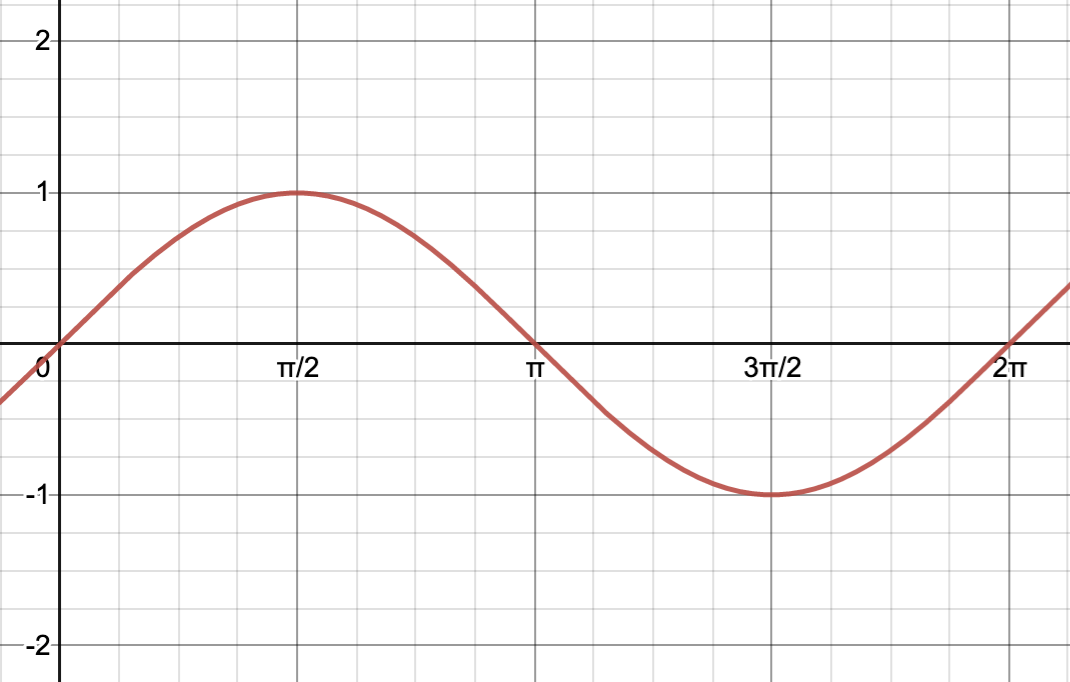
\includegraphics[width=0.5\textwidth]{figures/sine-wave-form.png}
	\caption{A basic sine wave}
	\label{fig:basic-sine-wave}
\end{figure}

\subsection{Sine Waves}\label{subsection:sine-waves}
The first of the basic period waves is the sine wave. The sine wave is a signal with only one frequency, and is based on the trigonometric sine function. On the unit circle, the trigonometric sine function of a phase angle $\theta$ is defined as the ratio of the length of the opposite side and the hypotenuse of a right triangle. The unit circle, with a radius of 1, results in the sine function $sin\theta$ being equal to the y-value in Cartesian coordinates, where the hypotenuse of the right triangle that is formed meets the circle, like in figure \ref{fig:unit-circle}. A trigonometric sine wave can then be used to synthesize a sine wave audio signal. So, instead of calculating the sine function for a single value $x$, to create the sine wave signal the sine function is performed on a time vector $t = \{t_1, t_2, \dots, t_n\}$, with units in seconds. $sin(t) = \{sin(t_1), sin(t_2), \dots, sin(t_n)\}$. This gives us what we see in figure \ref{fig:unit-circle}. The table below summarizes these transformations.

\begin{figure}
	\centering
	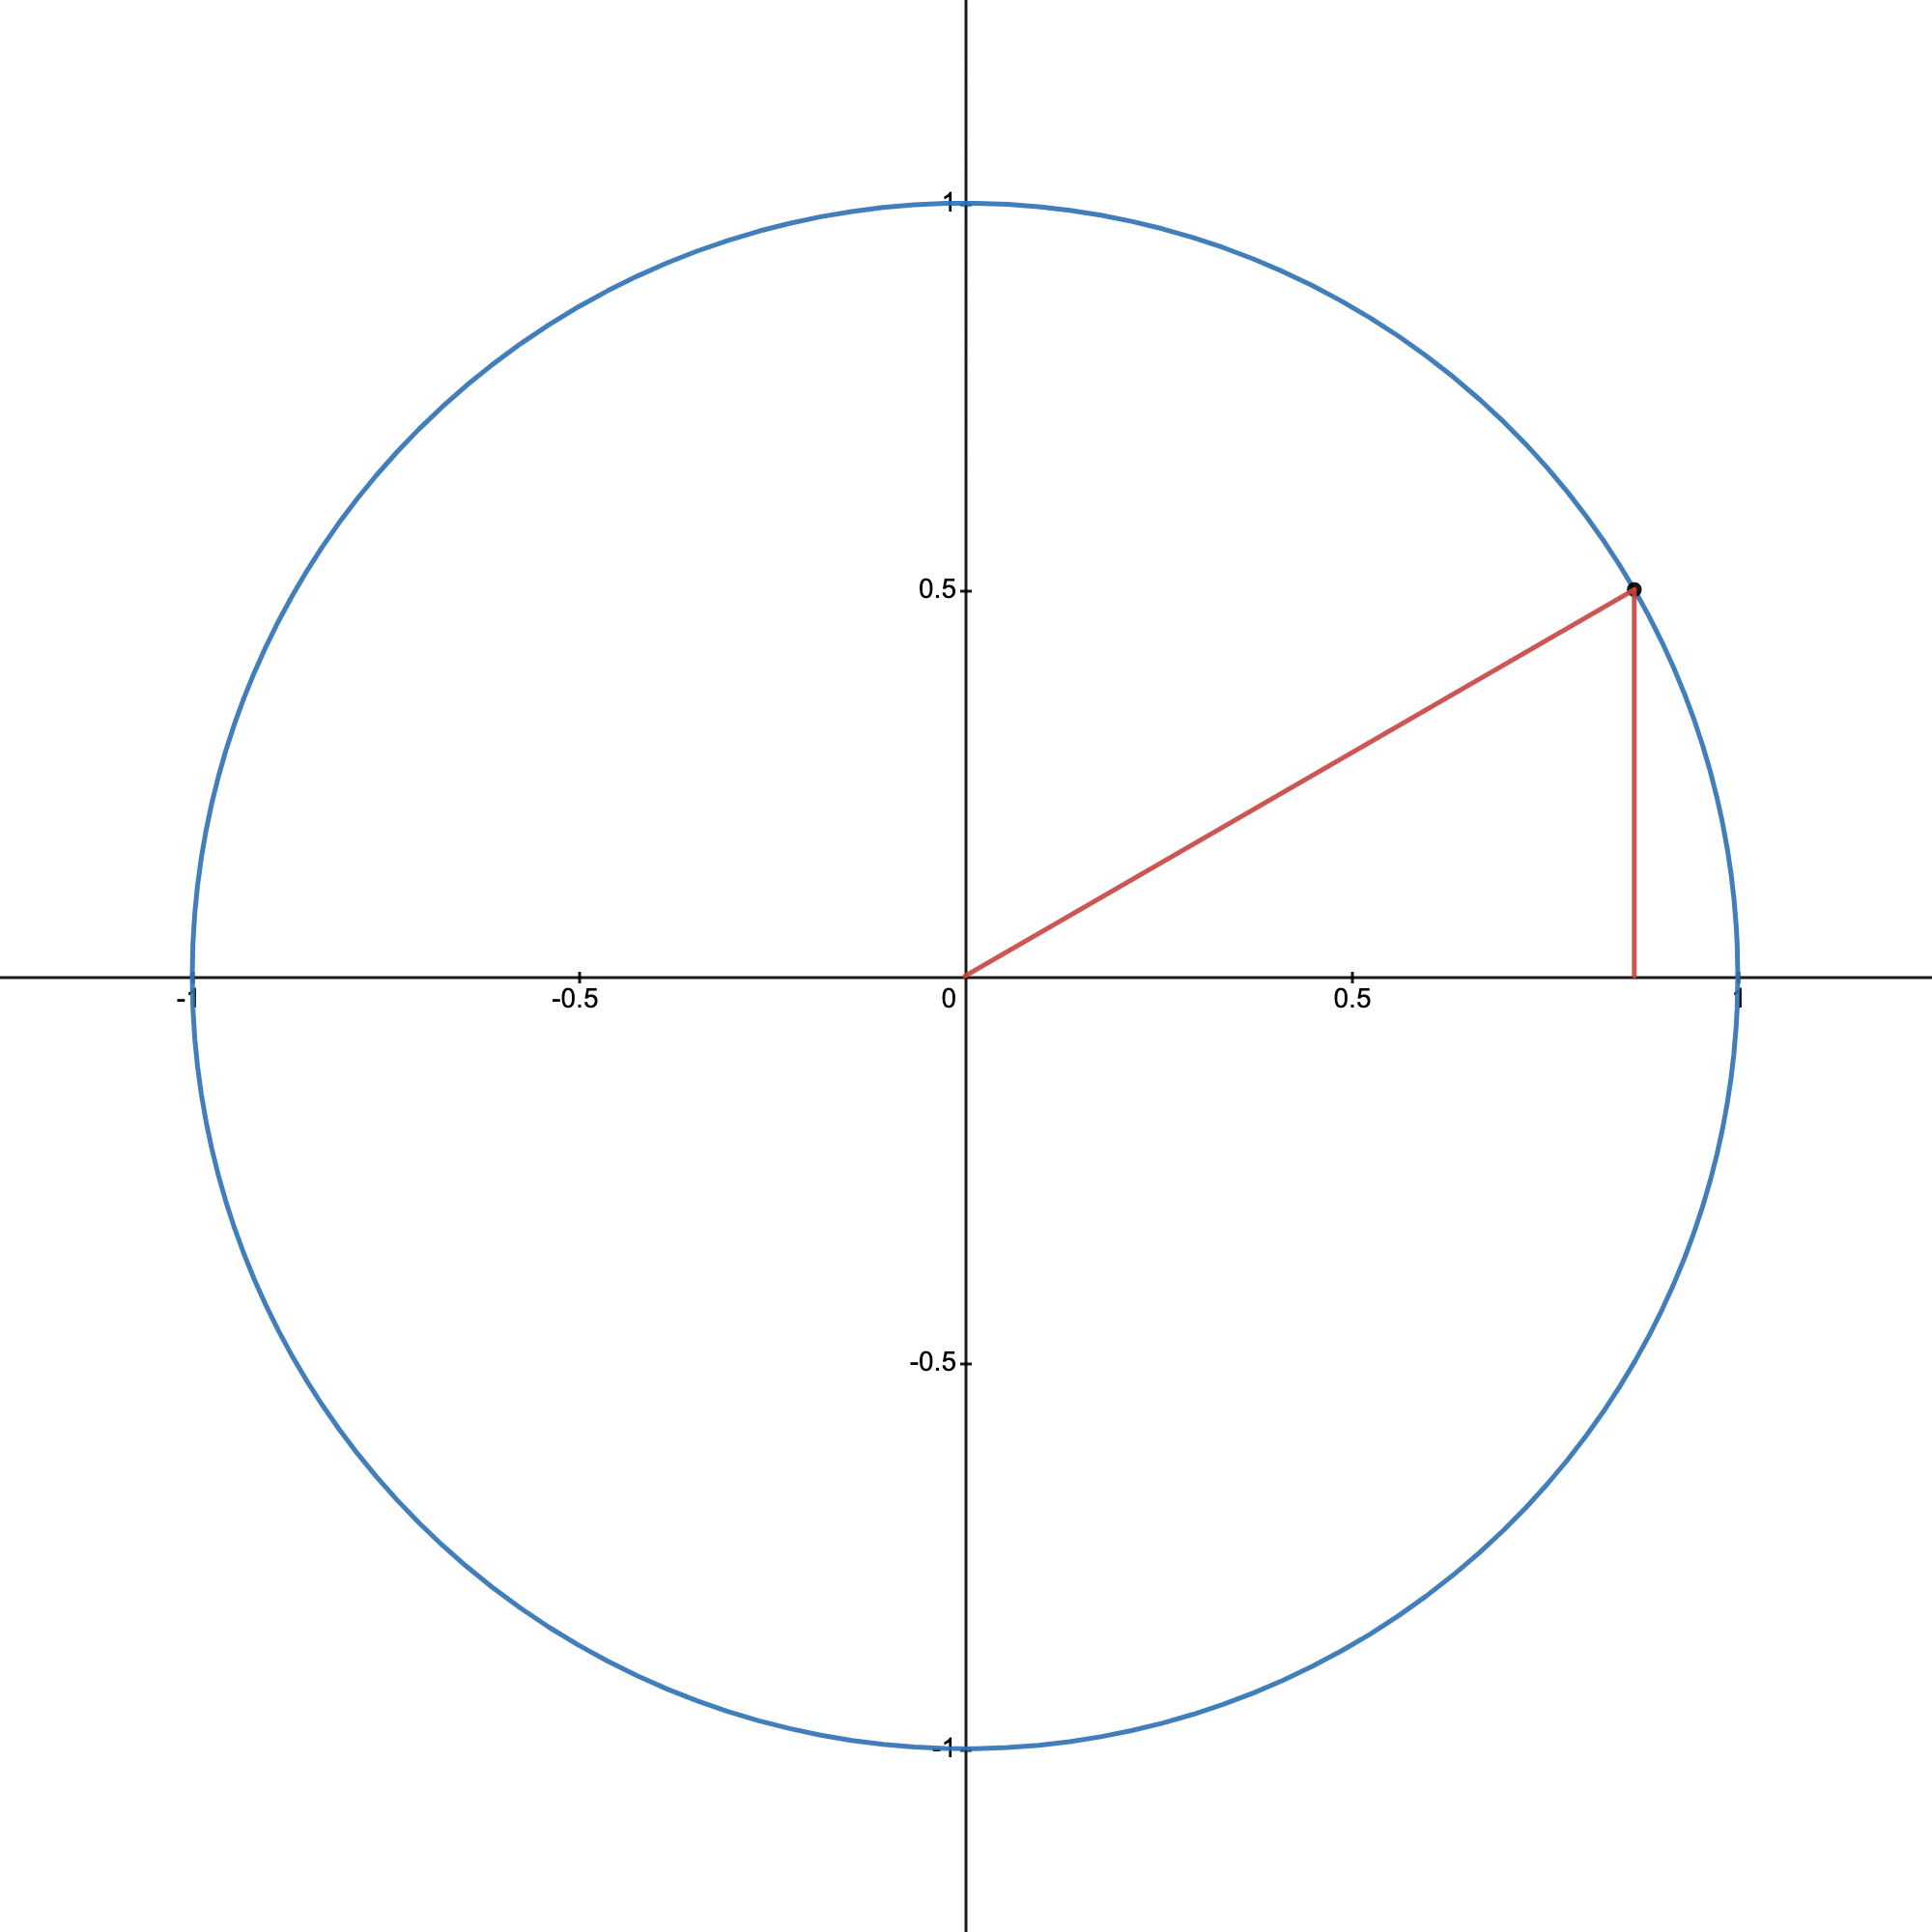
\includegraphics[width=0.5\textwidth]{figures/unit-circle.png}
	\caption{The unit circle}
	\label{fig:unit-circle}
\end{figure}

\begin{center}
    \begin{tabular}{c c}
        Function Input & Output Characteristics \\
        $sin(t)$ & $\frac{1 \textrm{ cycle}}{2\pi \textrm{ seconds}}$\\
        $sin(2\pi \cdot t)$ & $\frac{1 \textrm{ cycle}}{1 \textrm{ second}}$\\
        $sin(2\pi \cdot f \cdot t)$ & $\frac{f \textrm{ cycles}}{1 \textrm{ second}}$\\
        $sin(2\pi \cdot f \cdot t + \varphi)$ & Phase offset, $\varphi \varepsilon$ $[0, 2\pi]$\\
        $A \cdot sin(2\pi \cdot f \cdot t + \varphi)$ & Amplitude, \textit{A}
    \end{tabular}
\end{center}
The resulting sine wave signal can then be written as $x[t] = A \cdot sin(2 \cdot \pi \cdot f \cdot t + \theta$. $f$ is the frequency scalar, $t$ is the time vector of samples, and $\theta$ is the phase offset, between $[0, 2\pi]$.

\subsection{Square Waves}
The second of the periodic waves, the square wave, is a signal which oscillates between a singular positive value, and a single negative value \cite{Tarr_2019}. As seen in figure \ref{fig:square-wave}, the waveform itself is only ever positive or negative 1. An approximation of a square wave can be creating by combining multiple individual harmonics, or sine functions. This method of forming an audio signal is known as \textit{additive synthesis}, in which a new timbre is created by adding together sine waves. As a square wave is the summation of the odd-numbered harmonics, the following equation can be used \cite{Tarr_2019}.

\begin{figure}
  \centering
  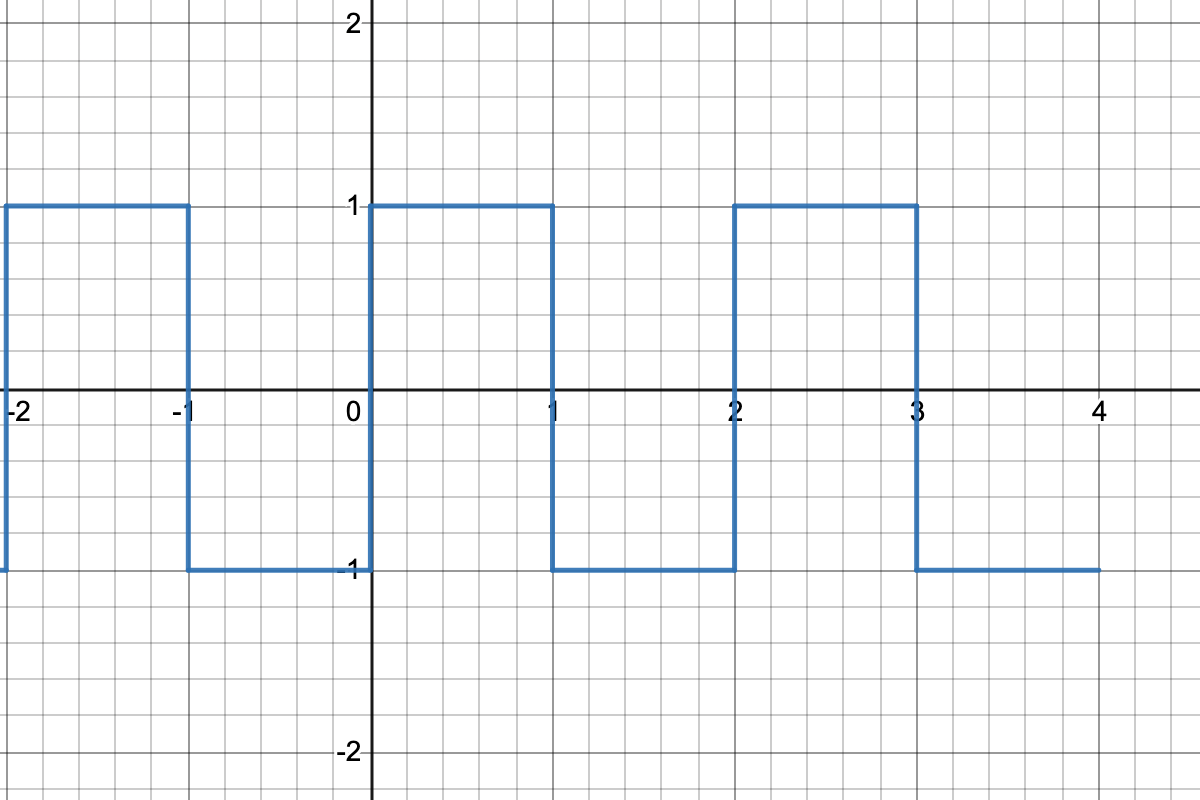
\includegraphics[width=0.5\textwidth]{figures/square-wave.png}
  \caption{A basic square wave}
  \label{fig:square-wave}
\end{figure}


\begin{align}
    \textrm{Let } x &= 2 \cdot \pi \cdot f \cdot t \\
    M &= \bigg \lfloor \frac{F_s}{2 \cdot f} \bigg \rfloor \\
    \textrm{square}(x) &= \frac{4}{\pi}(sin(x) + \frac{1}{3}sin(3 \cdot x) + \frac{1}{5}sin(5 \cdot x) + \dots) \\
    \textrm{square}(x) &= \frac{4}{\pi}\sum_{n=1, 3, 5, \dots}^{M}(n \cdot x)
\end{align}

Thus, the value \textit{M} is the harmonic with the highest frequency. This is calculated to be the number of odd harmonics less than the Nyquist frequency of $\frac{F_S}{2}$, rounded down to the nearest whole number. [INSERT DEF OF NYQUIST FREQ]

\subsection{Sawtooth Waves}
A Sawtooth wave is a signal with an amplitude which changes linearly between a minimum value, and a maximum value, as in figure \ref{fig:basic-sawtooth-wave}. Sawtooth waves are also created through additive synthesis, combining multiple sine functions together to create it. We have a similar equation to the one for square waves. 

\begin{figure}
  \centering
  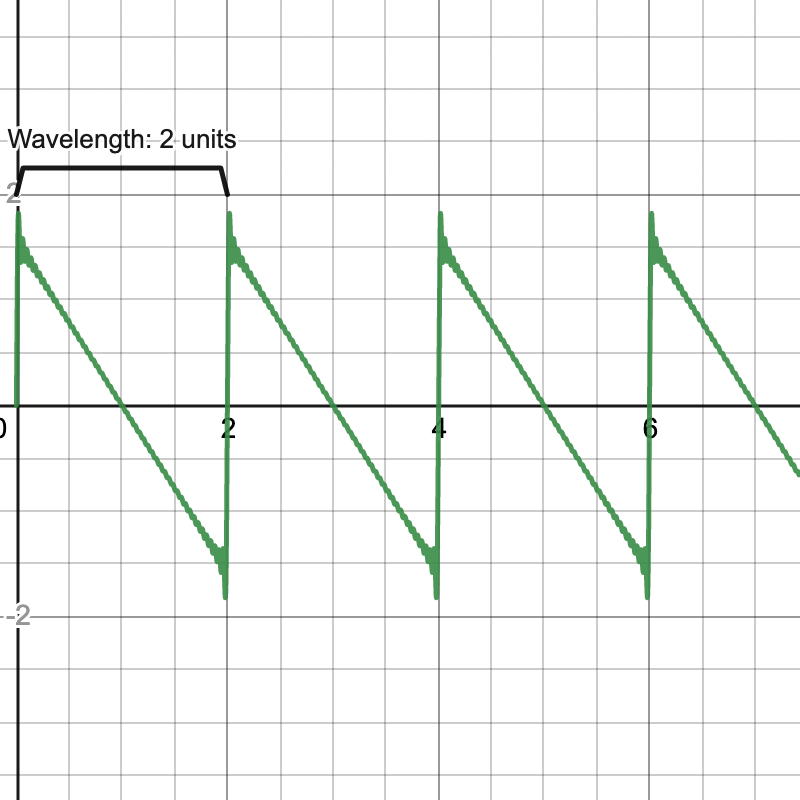
\includegraphics[width=0.5\textwidth]{figures/sawtooth-wave.png}
  \caption{A basic sawtooth wave}
  \label{fig:basic-sawtooth-wave}
\end{figure}


\begin{align}
    \textrm{Let } x &= 2 \cdot \pi \cdot f \cdot t \\
    M &= \bigg \lfloor \frac{F_s}{2 \cdot f} \bigg \rfloor \\
    \textrm{square}(x) &= \frac{1}{2} - \frac{1}{\pi}(sin(x) + \frac{1}{2}sin(2 \cdot x) + \frac{1}{3}sin(3 \cdot x) + \dots) \\
    \textrm{square}(x) &= \frac{1}{2} - \frac{1}{\pi}\sum_{n=1}^{M}(\frac{1}{n}sin(n \cdot x)
\end{align}

One thing to notice, is the equations for saw tooth waves and square waves are very similar, with both waves being the summation of the odd harmonics of the fundamental frequency \cite{Tarr_2019}.

\section{Time Domain and Frequency Domain}

Digital signals are studied in one of four domains: time domain, spatial domain, frequency domain, and wavelet domain. For the purposes of this research, we focus most on only two of these domains: the time domain and the frequency domain. These domains are most commonly used in audio analysis and synthesis. Digital audio is normally viewed in the time domain, and through the use of the Discrete Fourier Transform (sometimes also called the Fast Fourier Transform), we are able to produce a frequency domain representation for frequency analysis.

\subsection{Time Domain}

Audio is most commonly represented as a waveform, most commonly as the sine wave, with time plotted against the wave's amplitude. The x-axis will represent the discrete audio signal, and is normalized to represent the hours, minutes, or seconds. Normalization is the process of transposing a data set to a specific reference value, by dividing the output value by a given constant \cite{Zjalic_2021}. In audio, the most common type of normalization will be applied to a common audio waveform, to produce a signal that is normalized between the values of 1 and -1. 1 thus becomes the reference value for positive values, and -1 for negative values. To normalize audio, the following formula is applied to an audio signal: sample value $\times$ $\frac{1}{\textrm{reference value }}$. Audio normalization is useful for audio analysis, in that it allows for comparisons to be made between signals, regardless of their magnitude and sample rate \footnote{[INSERT DEF OF SAMPLE RATES]}. The y-axis then represents the magnitude of each audio sample, in which the decibels (or another magnitude unit) are a bipolar normalized value, between a positive and negative value. 

To transform the time representation from samples to seconds, the sample rate must first be known. From there, it is simple to transpose \cite{Zjalic_2021}. For example, we assume that for the 44100 samples we have that the sample rate is also 44100 Hz [INSERT DEF OF HZ IF NOT IN ALREADY]. So, $44100 / 441100 = 1$ second, in that we divide the number of samples by the sample rate, to obtain a time representation in seconds. Another example may showcase this better. Assume we have 2646000 samples, and a sample rate of 44100 Hz. Then, we have $2646000/44100 = 60$ seconds.

\subsection{Frequency Domain}
The physical concept of frequency is relatively simple: it is the number of occurrences per unit of time in a given phenomenon \cite{Gabrielli_2020}. In audio, this becomes the number of repetitions, or cycles, of a sine wave. This type of frequency is known as the \textit{temporal frequency}, and will be denoted with the letter \textit{f}. For acoustic audio signals, we will be describing frequency in Hertz (H).\footnote{The reciprocal of the temporal frequency is known as the period, denoted as capital \textit{T}. This is defined as the time required to completed one full cycle at any given frequency, otherwise known as $T = \frac{1}{\textit{f}}$.} In digital signal processing, we instead will be using angular frequency (radians per second, denoted with $\omega$), which measures the angular displacement per unit of time. Thus, we have the following relation between temporal frequency, angular frequency, and period \cite{Gabrielli_2020}.

\begin{align}
    f &= \frac{\omega}{2\pi} &w &= 2\pi &f &= \frac{2\pi}{T}
\end{align}

To convert a signal into the frequency domain, and to obtain its frequency components, the Fourier Transform can be used\footnote{The Inverse Fourier Transform can be used to go from the frequency domain to the time domain.}. Transforms like these are common in audio signal processing. These are mathematical operations which allow you to observe a signal from a different perspective\footnote{The result of a transform on an audio signal can be seen in figure 2.9 of Gabrielli.}.

\section{The Fourier Transform}
Joseph Fourier (1768-1830) stated that all sounds could be represented by one or more sine waves of various frequencies, amplitudes, durations, and phases. Any sound could then be broken down into its component parts, and analyzed with Fourier analysis \cite{Winer_2018}. 

The Fourier transform converts the time information to a magnitude and phase component of each frequency. With the Fourier transform, Fourier stated that any signal \textit{x} of time length \textit{t} can be broken down into the sine and cosine waves of which it is composed \cite{Zjalic_2021}, each having \textit{t} cycles. Thus, based on the properties of the specific audio signal, the Fourier Transform can be broken into four methods:

\begin{enumerate}
    \item Fourier Transform: applies to continuous signals which are aperiodic (without periodic repetitions)
    \item Fourier Series: applies to continuous, periodic signals
    \item Discrete Time Fourier Transform: applies to discrete signals\footnote{A signal which is defined at discrete points between positive and negative values} which are also aperiodic
    \item Discrete Fourier Transform: applies to discrete signals which are also periodic
\end{enumerate}

Digital data, and so digital audio, has no relation to the first two methods. Sine and cosine waves in audio are defined from negative to positive infinity, but it is impossible to be able to define these signals continuously. Instead, we must obtain the discrete values of these waves at each specific time point, inferring the information between these points. So, by imagining a sine or cosine wave as simply one repetition of a series of a periodic sinusoidal, the criteria for a Discrete Fourier Transform is met \cite{Zjalic_2021}. Thus, it is the only transform that is applicable to digital audio signal processing, as it is both discrete and periodic.

\subsection{Discrete Fourier Transform}
The Discrete Fourier Transform (or DFT) takes the audio samples in the time domain as an input, and outputs two frequency domain outputs: $\frac{N}{2} + 1$ points. These outputs represent the amplitude of the sine and cosine waves, with \textit{N} the number of samples in the input, giving us equation \ref{eq:dft-equation} below \cite{Gold_Morgan_Ellis_2011}. This equation is of a finite duration sequence x(n)
with $0 \leq n \leq N + 1$ \cite{Broughton_Bryan_2008}.

\begin{equation}\label{eq:dft-equation}
    X[k] = \sum_{k=0}^{N-1}x[n]e^{-j (\frac{2\pi}{N})kn}
\end{equation}

The Discrete Fourier Transform represents the vector $x[n]$ as a combination of harmonically-related sinusoidals. 

\subsection{Inverse Fourier Transform}
We can take the same concept found in the Discrete Fourier Transform, and apply it to its inverse. With the Inverse Fourier Transform, audio samples in the frequency domain and taken as input, and samples in the time domain are output. As seen in equation \ref{eq:inverse-fourier-transform-equation}, the equations for the Discrete Fourier Transform (DFT) and the Inverse Discrete Fourier Transform (IDFT) are similar. 
\begin{equation}\label{eq:inverse-fourier-transform-equation}
	x[n] = \frac{1}{N}\sum_{k=0}^{N-1}X[k]e^{-j(\frac{2\pi}{N})kn}
\end{equation}

\section{Audio Manipulations}
As previously mentioned in section \ref{section:modular-synth-what-is}, modular synthesis involves sending an audio signal through patches or modules in a linear format to achieve the desired sound output changes. To explain how these changes occur to a sound wave, we begin with a simple sine wave, as in figure \ref{fig:sine-wave-period-amplitude}. Sine waves are a waveform which is a function of time \texttt{t}:

\begin{figure}
	\centering
	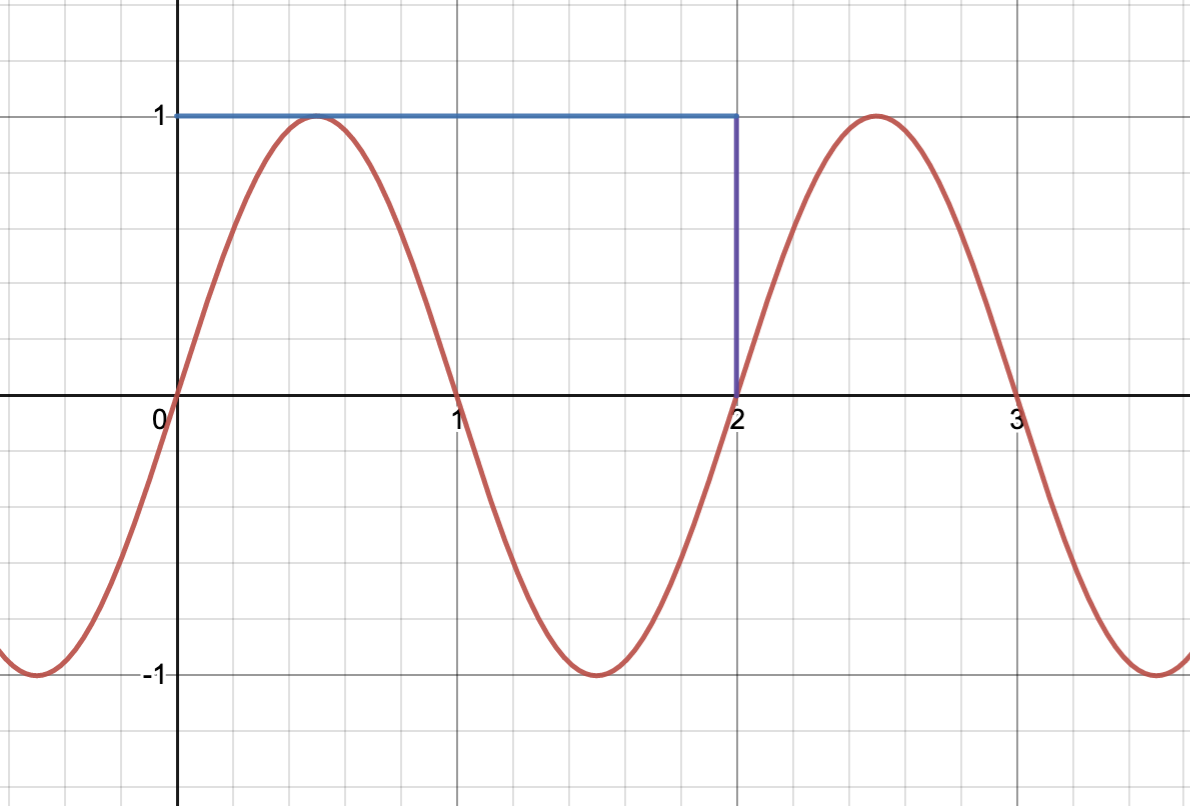
\includegraphics[width=0.5\textwidth]{figures/sine-wave-period-amplitude.png}
	\caption{A basic sine wave, with period demarcated in blue, and amplitude in purple}
	\label{fig:sine-wave-period-amplitude}
\end{figure}

\begin{equation}\label{eq:full-sine-wave-equation}
	y(t) = A \sin(2\pi ft + \varphi) = A\sin(\omega t + \varphi)
\end{equation}

with variables $A$, $f$, $\omega$, $\varphi$. $A$ is the wave's amplitude, which determines the peak deviation from zero. $f$ is the temporal frequency. $w = 2\pi f$ and is the angular frequency, and $\varphi$ is the wave's phase, which specifies (in radians) where in its cycle the wave's oscillation is at time $t = 0$ \cite{Kirk_Hunt_2013}. When $\varphi$ is not equal to zero, the wave itself will appear to be shifted by the value equal to $\varphi / \omega$, which is known as a wave's \say{phase shift}. A negative value will represent a delay in sound, while a positive value will represent an advance in the heard sound.

Thus, there are three primary options when manipulating audio (or a simple waveform); amplitude, frequency, and phase can all be modified at various points to affect the audio output. The first, amplitude, will determine the volume of the wave's sound. The larger the distance between zero and the wave's peak, the higher the human ear will perceive the sound to be\cite{Zjalic_2021}. In figure \ref{fig:sine-wave-period-amplitude}, amplitude is colored purple, and we see it has a value of 1 (the default value of amplitude of a sine wave from the unit circle), as $A$ does in equation \ref{eq:full-sine-wave-equation}. By changing the value of $A$ to either $\frac{1}{2}$, or $2$, the peak of the wave will change accordingly, becoming larger or smaller depending on the set value of $A$. This change is reflected in the sound we can hear, as like in figure \ref{fig:half-sized-sine-wave} and equation \ref{eq:half-sized-sine-wave}, the volume of this sine wave is halved.

\begin{equation}\label{eq:half-sized-sine-wave}
	y(t) = \frac{1}{2} \sin(\omega t + \varphi)
\end{equation}

\begin{figure}
	\centering
	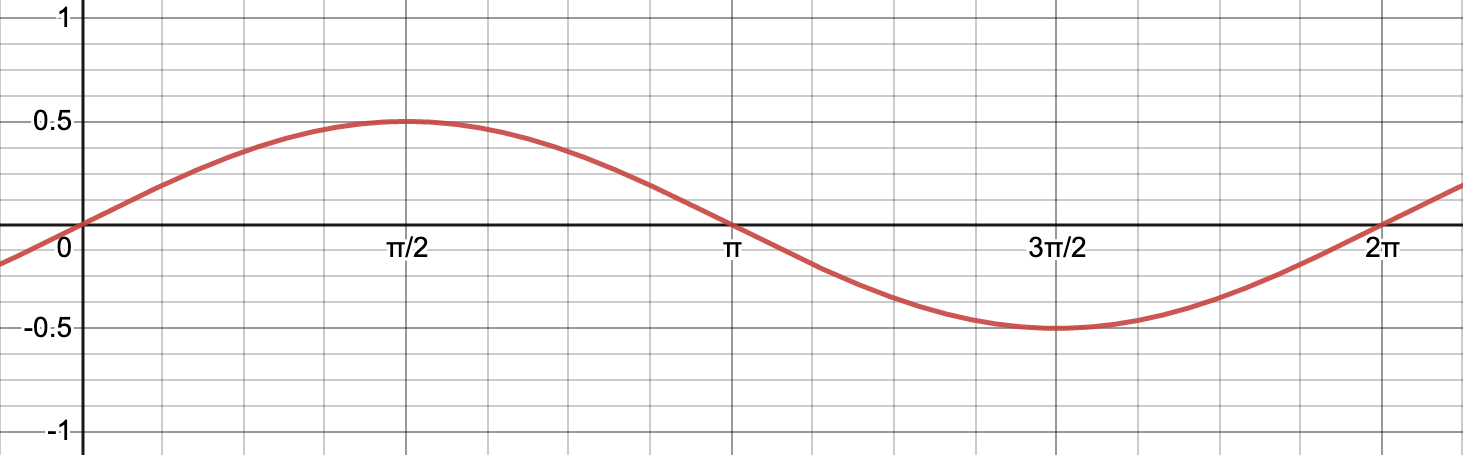
\includegraphics[width=\textwidth]{figures/half-sized-sine-wave.png}
	\caption{A sine wave, with an amplitude of $\frac{1}{2}$}
	\label{fig:half-sized-sine-wave}
\end{figure}

The second option commonly used to manipulate audio is to change an audio signal or wave's temporal frequency. For sound and audio manipulations, the temporal frequency component determines a sound's \say{color}, or \say{timbre}. It is the property of a waveform which determines the output sound's pitch. The high-end of audible frequencies for the human ear is around 20,000 Hz (20 kHz), though this reduces with age. The generally accepted range of human hearing ranges from 20 Hz to 20 kHz, with frequencies below 20 Hz felt more than heard\cite{Rosen_Howell_2011}. This range is further broken down in table \ref{tbl:frequency-table-of-human-hearing-general}. Thus, with equation \ref{eq:full-sine-wave-equation}, we change the value of $f$, which will alter the frequency of the wave, and then also alter the perceived pitch. With an increase in temporal frequency, there will also be an increase in angular frequency $\omega$, which increases the rate of change of the sine wave. With the period of the sine wave in figure \ref{fig:sine-wave-period-amplitude} marked blue, it is this blue section that will increase with an increase in $\omega$. As $\omega$ increases, there are more repetitions of the sine wave's phase, so the audio output's pitch will increase.

\begin{table}
	\begin{tabular}{|p{20em} | p{25em}|}
		\hline
		General Frequency Range & Description of Range \\ 
		\hline
		<20Hz - 60Hz & The lowest threshold of human hearing. This includes many frequencies that are felt and not heard, and provides the \say{rumble} feeling in music. This range gives much of music its power, and is typically known as \say{sub-bass}. \\
		\hline
		60Hz - 250Hz & This range determines the amount of \say{warmth} and how full the sound is perceived to be. The notes fundamental to rhythm lives in this range, and too much sound in this frequency range will result in the overall sound being \say{boomy}, or muddy-sounding and messy. It is otherwise known as the the \say{bass} frequency. \\
		\hline
		250Hz - 500Hz & The lower harmonics of many instruments are in this range. It is generally known as the \say{lower midrange} of frequencies, and can introduce listening fatigue and a telephone-quality to the sound if this range is emphasized too much. \\
		\hline
		500Hz - 2 kHz & This range is considered the middle of the midrange. It gives many instruments prominence in a mix, and determines how audible one instrument or vocalist is in comparison to another. If this range is emphasized, audio output may sound tinny and small, which could lead to listening and ear fatigue, as the human ear is sensitive to the human voice, and the frequencies it covers. \\
		\hline
		2 kHz - 4 kHz & The \say{upper midrange} is responsible for much of the attack sounds on percussive and rhythmic instruments. This range may add presence to the mix if boosted, but if it is emphasized too much, it may mask some speech recognition sounds. Listening fatigue may also set in if this range is emphasized too much, as the slightest boost in this range will result in a noticeable change in the sound's timbre. \\
		\hline
		4 kHz - 6 kHz & This range is known as the \say{presence} range. It defines a sound's clarity and the definition of voices and instruments that are present. If this range is boosted, instruments and voices may sound physically closer to the listener, and vice versa, with reducing this range causing instruments and voices to sound further away. However, if this range is emphasized too much, a harsh, irritating sound may occur. \\
		\hline
		6 kHz - 20 kHz & This range controls the \say{brilliance} and clarity of sounds within the mix. Instead of pitches, this range is composed entirely of harmonics, and brings \say{sparkle} to the sound. This range also may easily cause ear fatigue, as an over-emphasis can increase the hiss heard, and produce sibilance, or an unpleasant tonal harnshness which can happen with consonant syllables (most noticeably: S, T, and Z), especially on vocals. \\
		\hline
	\end{tabular}
\caption[A description of the human hearing range]{Descriptions of general frequencies ranges within the range of human hearing}
\label{tbl:frequency-table-of-human-hearing-general}\cite{Suits_1998}\cite{Zjalic_2021}
\end{table}

Finally, a modification to a wave's phase will determine if the audio signal output is on-time, delayed, or early. The numeric value of $\varphi$ depends on the start of the wave's period. Similar to the changes made to amplitude and frequency, by modifying the value of $\varphi$, we change the phase of the waveform. This will be most noticeable with multiple harmonics or simple waveforms stacked on top of each other, in which each signal will have a phase at a slightly different time, as in figure \ref{fig:sine-wave-phase-shift}. The period of the blue sine wave has a length of $\frac{\pi}{2}$, but otherwise is a normal unit circle sine wave. The red sine wave is phase shifted, with a $\varphi$ value of positive 2, which shifts the wave negative, causing the output audio to sound early in comparison to the blue wave. 

\begin{figure}
	\centering
	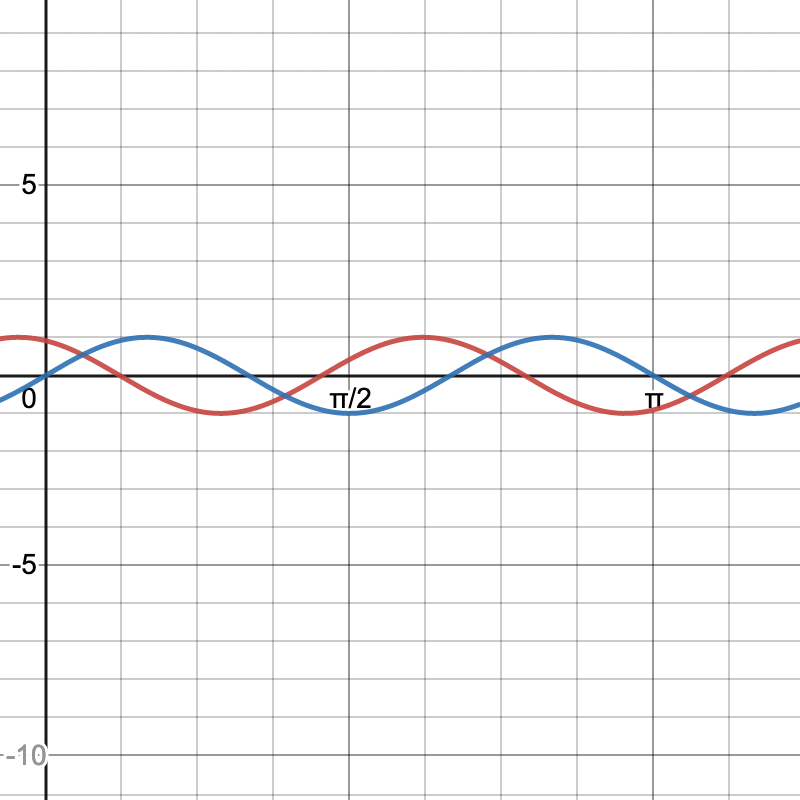
\includegraphics[width=0.5\textwidth]{figures/sine-wave-phase-shift.png}
	\caption{The phase shift in a sine wave}
	\label{fig:sine-wave-phase-shift}
\end{figure}

These three changes to an audio waveform will be the basis for the modules created in this project, in which some combination of modifications made to the audio signal will produce the desired changes. 